\chapter{Analisi statica}

\section{Struttura binari}

\subsection{ELF}

\subsection{PE}
Potrebbero essere offuscati, come vedremo più avanti

\section{IoC: Indicator of Compromise}

\section{Capa: capabilities}
Includere anche il test su Colab con le statistiche.

\section{Yara: signature-based}
Sia per statici che in memoria dei processi.

Ora però usate solo per analizzare staticamente un file eseguibile.

\section{File offuscati}
Packed, installer, ... come li trattiamo?

Analisi rimandata alla parte dinamica, perché lì possiamo sfruttare altri strumenti di analisi integrati in Cuckoo, più potenti di quello che potremmo fare manualmente qui.

Ci basta avere i dati di ciò che stiamo trattando, ad esempio l'output in questo caso sarà del tipo:
\begin{code}
\captionof{listing}{Output CAPA su file packed}
\label{code:json_capa_packed}
\begin{minted}{json}
{
    "capa": {
        "format": "packed",
        "arch": "i386",
        "os": "windows"
    }
}
\end{minted}
\end{code}

Nessuna regola viene eseguita, perché \texttt{capa} non supporta questi formati per l'estrazione delle capabilities usando i propri strumenti integrati. \ref{code:json_capa_packed}

\section{Riconoscitore custom del tipo di file}
Partendo dalla necessità di velocizzare l'operazione di riconoscimento del file, in sostituzione dell'esecuzione del comando \texttt{capa -r anti-analysis} che può portare a richiedere diversi minuti a seconda del numero di funzioni presenti nel file, come visto in \textbf{FIGURA REF},
dobbiamo ricorrere a una diversa soluzione.

Dato che si tratta di un problema di enumerazione, non aveva senso andare a creare e mantenere un proprio riconoscitore di ogni possibile formato di un file. Ad esempio, già solo per quanto riguarda i file pacchettizzati, esistono tantissimi packer e tanti ne esisteranno in futuro.

Inoltre, spesso malware usano packer personalizzati, che hanno leggere differenze da quelli noti e si correrebbe il rischio di creare uno strumento poco efficace.
Per questi e altri motivi quali il tempo a disposizione, è stato scelto di usare come base uno strumento noto (\texttt{Detect-It-Easy}) per fare una prima analisi, affiancato da uno script Python custom che decide quali operazioni svolgere a seconda del tipo di file, va a fare il parsing del JSON dato in output e si integra nello script Bash creando un layer di astrazione col resto del workflow.
Infatti, nel caso servisse modificare lo strumento sottostante, sarebbe sufficiente adattare la traduzione dall'output specifico del tool al contratto stabilito col resto del programma per rendere seamless questa variazione, anche sostanziale.

Tuttavia, a fini di comprensione pratica del funzionamento dietro questo genere di detector, è stato creato un Proof of Concept, scritto in Python, in grado di rilevare solo alcuni dei tipi dei più famosi packer come UPX, o se si tratta di un installer Inno-Setup, nei file PE x86\_64 (Windows).
Sono state usate caratteristiche note di questi packer
\footnote{\url{https://github.com/mandiant/capa-rules/tree/e88db21de4d4cf9f7abec9177fab11240075036b/anti-analysis/packer}}
per eseguire la detection, sfruttando la libreria pefile per non eseguire l'intero parsing a mano dei byte degli header e non essere dipendenti da implementazioni native dell'OS come con l'uso dell'header \texttt{windows.h} in un programma C.

\begin{figure}[h!]
    \centering
    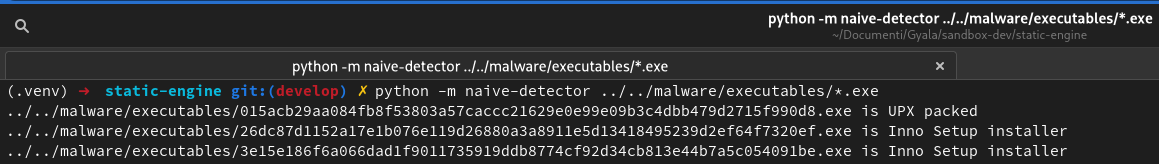
\includegraphics[scale=0.34]{assets/custom_file_detector_output.png}
    \caption{Custom file detector output}
\end{figure}

\subsection{UPX}
Le regole più comuni
\footnote{\url{https://github.com/mandiant/capa-rules/blob/e88db21de4d4cf9f7abec9177fab11240075036b/anti-analysis/packer/upx/packed-with-upx.yml}}
per riconoscere UPX impongono di leggere le sezioni, e vedere se queste contengono \texttt{UPX0} o \texttt{UPX1}.

Facciamo una comparazione tra la regola capa per il rilevamento e il codice del riconoscitore.

\noindent\begin{minipage}{.35\textwidth}
       \begin{minted}{yaml}
features:
    - format: pe
    - or:
      - section: UPX0
      - section: UPX1
       \end{minted}
\end{minipage}
\begin{minipage}{.4\textwidth}
       \begin{minted}{python}
def is_upx(file_path):
    file_sections = get_section_names(file_path)
    upx_sections = [ "UPX0", "UPX1" ]
    for upx_section in upx_sections:
        if upx_section in file_sections:
            return True
    return False
       \end{minted}
\end{minipage}

\bigskip

Andando però a sfruttare la libreria Python per il parsing del file PE senza ricorrere a implementazioni native Windows:

\begin{minted}{python}
import pefile

def get_section_names(file_path):
    pe = pefile.PE(file_path)
    sections_set = {
        section.Name.decode().strip().strip('\x00')
        for section in pe.sections
    }
    pe.close()
    return sections_set
\end{minted}

\subsection{Inno-Setup Installer}
Con Inno-Setup, possiamo notare come sia ancora più semplice il riconoscimento. Infatti, non abbiamo bisogno di andare a vedere le sezioni, ma è sufficiente controllare la presenza di alcune stringhe statiche nel file.

Nuovamente, andiamo a paragonare la regola capa alla nostra implementazione:

\begin{minted}{yaml}
features:
    - and:
      - string: /^Inno Setup Setup Data \(/
      - string: /^Inno Setup Messages \(/
\end{minted}

\begin{minted}{python}
def is_innosetup(file_path):
    BUFFER_SIZE = 65536
    with open(file_path, 'br') as f:
        match_setup, match_messages = False, False
        buffer = f.read(BUFFER_SIZE)
        overlap = len(b'Inno Setup Setup Data (')

        while len(buffer) > overlap and (not match_setup or not match_messages):
            # Match inside current buffer
            if not match_setup and b'Inno Setup Setup Data (' in buffer:
                match_setup = True
            if not match_messages and b'Inno Setup Messages (' in buffer:
                match_messages = True
            
            # Read next buffer, allowing for overlap
            buffer = buffer[-overlap:] + f.read(BUFFER_SIZE)
    
    return match_setup and match_messages
\end{minted}

\section{FLARE Floss}
Teoria: \url{https://github.com/mandiant/flare-floss/blob/master/doc/theory.md}

\section{Automazione su AWS}
\subsection{Scrittura dei parser}
Parser per capa e yara.

Parser dal file testuale, con schemini.


\subsection{Creazione dell'immagine}
Prima era enorme (naive approach), poi ridotta sfruttando il multistage

\subsection{Workflow di analisi statica}
Upload su S3, poi risultato nel db

\subsection{Deploy su AWS}
Immagine dell'architettura (SVG)

Sicurezza e varie policy (hardening)